%%
%% Author: thompson
%% 02.11.17
%%

% Preamble
\documentclass[11pt]{article}

% Packages
\usepackage{a4wide}
\usepackage{verbatim}       % Package for "Sourcecode"
\usepackage{scrextend}
\usepackage{enumerate}
\usepackage{graphicx}


% FIXME: Linkreferences by footnotes are buggy
% Document
\begin{document}
    \section{JS and DOM Basics}
    \begin{enumerate}[\thesection .1]
        \item What is the purpose of Javascript and how does it complement HTML and CSS?\footnote[1]{Src.: $https://www.w3schools.com/js/js\_whereto.asp $}\\
        Javascript gilt als Programmiersprache, ähnlich wie Java, Rust, php, ....
        Javascript wird mithilfe des $<$script$>$-Tags in ein HTML-Dokument eingebunden.
        Ein externales sowie internales Einbinden von Javascript ist zu jeder Zeit möglich, egal ob es sich dabei um Sourcecode
        innerhalb des Head oder des Body befindet. (Siehe demoHTML.html)

        \begin{verbatim}
        <!DOCTYPE html>
          <html>
            <head>
            <script src="demoJS.js"></script>
            </head>

            <body>
              <h1>A Web Page</h1>
              <p id="demo">A Paragraph</p>
              <button type="button" onclick="myFunction()">Try it</button>

            </body>
          </html>
        \end{verbatim}
        Mithilfe von JS lassen sich Funktionen effizient schreiben.
        Es gilt dabei zu beachten, dass es zu den guten Praktiken gehört, JS-Code von HTML und CSS zu trennen.
        Dementsprechend ist ein externales Einbinden anstrebbar.
        \begin{enumerate}
            \item[$\diamond$] Vorteile und Nachteile von Internen Code
            \begin{enumerate}
                \item[+] Schnelles Testing \& Debuggen
                \item[-] Lange Quellcodes führen zu unübersichtlichen Code
                \item[-] Langer Wartungsaufwand bei dupliziertem Quellcode
            \end{enumerate}

            \item[$\diamond$] Vorteile und Nachteile von Externem Code
            \begin{enumerate}
                \item[+] Übersichtlicher Code
                \item[+] Kurzer Wartungsaufwand
                \item[+] Zwischengespeicherter JS-Code beschleunigt Ladezeiten
            \end{enumerate}
        \end{enumerate}

        \item What kind of typing is provided by Javascript? What are the risks? \footnote[2]{Src.: $https://www.w3schools.com/js/js\_type\_conversion.asp$}\\
        In Javascript unterscheidet man zwischen folgenden
        \begin{addmargin}[1em]{1em}
            Typen:
            \begin{enumerate}[$\circ$]
                \item String - Die allbekante Zeichenkette in "Text"
                \item Number - Eine beliebige Zahl mit/ohne Nachkommazahlen
                \item Boolean - Ein Wahrheitswert, True oder False
                \item Object - Ein Objekt, ähnlich einer Klasse in Java
                \item Function - Eine Funktion, etwa fn(){}
                \item null - Ein Objekt ohne Wertzuweisung
                \item undefined - Ein nicht definiertes Objekt
            \end{enumerate}

            Objekten:
            \begin{enumerate}[$\circ$]
                \item Object - Ein Objekt, ähnlich einer Klasse in Java
                \item Date - Date() als eigene vordefinierte Klasse für die Zeit
                \item Array - Ein Array aus Werten.
            \end{enumerate}
        \end{addmargin}

        \item What is DOM?\\
        Dom, Document Object Model, beschreibt ein neutrales Interface zwischen .js und .html.
        Es soll dynamischen Zugang \& Update von Inhalt ermöglichen.
        Levels of DOM und DOM Level sind 2 unterschiedliche Spezifikationen:
        \begin{enumerate}[$\diamond$]
            \item Levels of DOM beschreibt die Hierarchie innerhalb eines Körpers. Beispielsweise gliedert sich
            \begin{verbatim}
                <p>Hello, <b>World</b>!</p>
            \end{verbatim}
            in $<$p$>$ := Level 1 und $<$b$>$ := Level 2

            \item DOM Level x beschreibt die derzeitig genutzte Norm für HTML-Standards.
            \begin{addmargin}[1em]{1em}
                - DOM Level 1: HTML \& XML Dokument-Model, inklusive Möglichkeit der Veränderung der Dokumente.\\
                - DOM Level 2: Eventmodel \& Funktionserweiterung "getElementById". Supporterweiterungen von XML und CSS.\\
                - DOM Level 3: Support für XPath, Keyboard-Event-Handling und Serialisierung von Dokumenten als XML.\\
                - DOM Level 4: Work in Progress, veröffentlicht 2015 als WHATWG living standard.
            \end{addmargin}
        \end{enumerate}

        Prinzipiell soll man mithilfe von Funktionsaufrufen via .js oder .php auf DOM-Objekte zugreifen.
        DOM-Objekte sind grundsätzlich spezifiziert im .html, wobei der Begriff "Objekt" auf die jeweiligen Tags abzielt.

        \begin{minipage}{0.5\textwidth}
            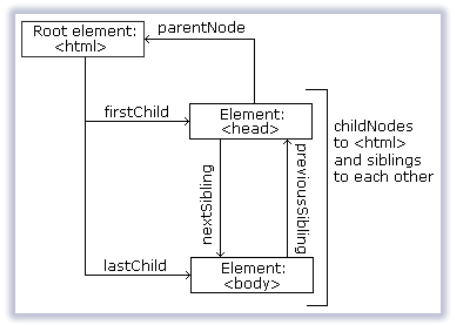
\includegraphics[width=1\textwidth]{DOM_js.png}
            .js Zugriffsdisplay innerhalb des DOM
        \end{minipage}
        \begin{minipage}{0.5\textwidth}
            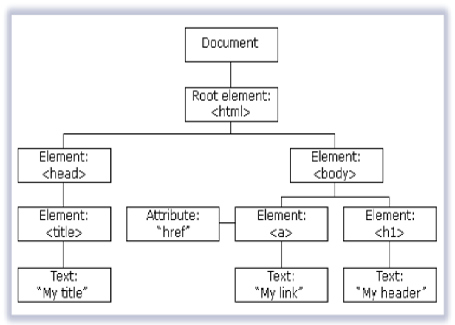
\includegraphics[width=1\textwidth]{DOM_html.png}
            Aufbau des DOM durch .html
        \end{minipage}
    \end{enumerate}

        \emph{Beispiel: Simple DOM-Tree Manipulation}
    \begin{verbatim}
        <!DOCTYPE html>
          <html lang="en">
            <head>
              <meta charset="UTF-8">
              <title>DOM-Manipulation Demo</title>
            </head>
            <body>
              <p style="color: green;"
                onmouseover="hoverStart(this);" onmouseout="hoverEnd(this);">
                Hover me!
              </p>
              <p style="color: green;"
                onclick="this.innerHTML='You clicked me!';">
                Click me!
              </p>

        <script src="demo_DOMscripts.js"></script>

        </body>
        </html>

        // Javascript below
        function hoverStart(element) {
        element.innerHTML='You hover me!';
        }
        function hoverEnd(element) {
        element.innerHTML='Thanks for not hovering me!';
        }
    \end{verbatim}

\end{document}